\chapter{Design}
\label{chap:design}

%In order to begin construction of the artifact it is necessary to understand the domain in which it should operate. To motivate design decisions we need to understand the domain data, what kinds of queries that will be done on this data as well as the overall architecture of the system. Once this understanding is reasonably adequate, designs decisions can be made with more confidence. However,  decisions should also take solution objectives into account. 

This chapter describes the design of the artifact and the constructed prototypes.

Through the review of related work, establishment has been made that non relational databases are appropriate as a part of a solution to the identified problem of this thesis. However, it has also been suggested \cite{NoSQLSurvey} that the introduction of non relational storage should not replace current relational databases, but should instead work as a complement. We argue that a polyglot persistence solution is a natural approach to the identified problem. Implementing such a solution would then address objective 1, namely to physically separate live from stale data. Before implementation, a decision has to be made on what types of databases should be used as the underlying storage for the archive. If the only objective was data separation then the simplest choice would be to completely duplicate system data in its current form to a similar database. However, this does not take into account other objectives and would likely not solve the underlying problem. 

When selecting what databases to use we need to address the previously established issue of evolving data (objective 3) and the need to minimize long running migrations of this data to new schema versions. One way this could be addressed is by using a database with a flexible schema, capable of handling heterogeneous data. Said database should also have query capabilities that allow us to effectively address objective 2; the retainment of important queries.

In order for the archive system to scale naturally with the current level of data growth (objective 4), it is prudent to select a database with horizontal scaling. In addition to this, it would be highly beneficial with more efficient data compression than what is currently in use by the relational database of CIMS.

Two different NoSQL databases and one relational database were selected to be used for the implementation of archive prototypes. They are described in more detail in the following sections.

\section{MongoDB}
The main motivation for choosing MongoDB as a candidate is its flexible data model along with custom indexes and extensive query capabilities \cite{Catell}. As a comparison, a key-value store would be to constricting for the types of queries that need to be supported by the archive as seen in table~\ref{tab:queries}. A document-store has, at least in theory, the right mix between data model flexibility and query capabilities. Our intent with this design choice is to evaluate the suitability of document-stores in general as a means to solve the identified problem. 

\section{Elasticsearch}
Elasticsearch is classified as a search engine, but has some similarities to MongoDB, such as its data model and the ability to scale horizontally. The difference is mainly in query capabilities, which in are optimized for full text search. However, supporting full text search comes at a price of higher demands on hardware. We believe this to be an interesting trade-off to consider, and a comparison between MongoDB and Elasticsearch should yield useful practical information on how to proceed with the development of an archive solution after the study has been conducted.

\section{NoSQL data model}
With the domain description as a basis, the schema of the relational database in CIMS should be transformed to suit the strengths of the chosen NoSQL databases. A level of denormalization is prudent since any relationship between collections in a document store has to be implemented in application logic. However, no relationships at all would not be suitable for the types of queries that need to be supported. As such, the data model of the archive needs to be well designed. Given the use of document-stores and their data model, one natural change is to convert one to many relationships into lists of embedded documents. Another change is to denormalize all one to one relationships.

To illustrate the transformation process, we present a diagram in figure~\ref{fig:nosql} describing a proposed non relational schema for the archive. This can be compared to the original relational schema in figure~\ref{fig:sql}.

\begin{figure}[h!]
\centering
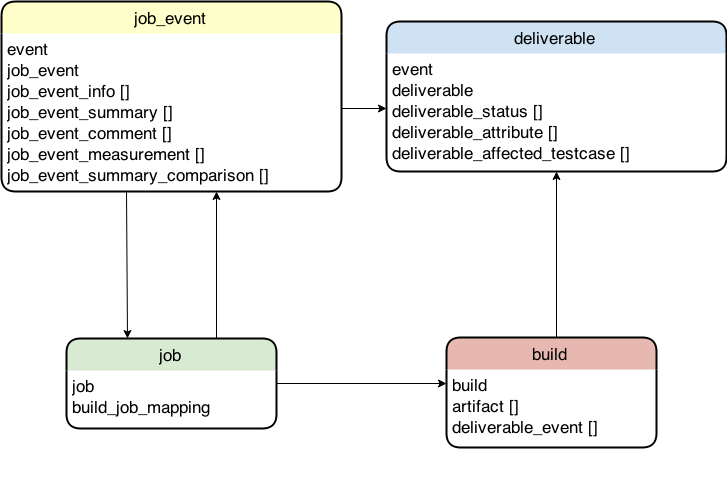
\includegraphics[scale=0.5]{figure/nosql.png}
\caption{Representation of the non-relational model. Bracket pairs represent a list of embedded documents.}
\label{fig:nosql}
\end{figure}

\section{TokuDB}
TokuDB is a storage engine for MySQL that aims to bring MySQL up to par with NoSQL databases in terms of scalability and flexiblity, while still retaining the ACID transactions that are common in relational databases. It does this by adressing many of weaknesses of MySQL and its most widely used storage engine, InnoDB. A much higher compression rate is achieved by leveraging fractal tree indexing. Schema migrations can be performed without locking the table.

An archive prototype will be developed using MySQL with TokuDB as the storage engine. This will provide a good contrast to the NoSQL based prototypes and has potential benefits that the NoSQL approach does not have. For example, the same schemas can be used for CIMS and the archive, making data transfer seamless between the two. However, the effectiveness of this solution is highly dependant on whether schema migrations are manageable with very large data sets.

\section{Software components}
A set of software components should be developed in order to effectively support the databases used for the archive prototypes. These components serve as glue code between the relational database of CIMS and the database of the archive. 

\subsection{Data migration tool}
Data needs to be extracted from the live relational database before it can be transformed and migrated elsewhere. This component should group data into chunks that makes sense to migrate as a unit.

\subsection{Data transformation tool}
After data has been extracted it should be transformed to fit the new schema in figure~\ref{fig:nosql}. The transformed data is then ready for insertion into the archive.

\subsection{Archive API}
To demonstrate the capability of the archive to respond to queries, an API should be developed that capture these queries. 

%\subsection{Schema evolution tool}
%To effectively support schema evolution, two features should to be implemented. The first is to effectively extract and transform data from different schemas of the relational database in CIMS. The second is to respond to queries that span multiple schema versions. These features will likely be extensions to the previously defined components.

%The artifact must be able to handle the evolution of the data in the archive, as previously stated it is not sure that all data will be accessed. A database solution that do not need to migrate all it's data to new schema versions could therefore be a viable solution. In a relational database, all data need to be homogeneous \cite{HittaEnSqlBok}, meaning all data must be in the same schema version. A NoSQL document store on the other hand is able to handle heterogeneous data \cite{NoSQLDistilled}, data with different structure.  

%\subsection{Choice of NoSQL databases}
%As stated in \cite{Catell, NoSQLSurvey, NoSQLDistilled, DbCrossroad} there exists different types of NoSQL stores with different use cases and purpose. A great variety of NoSQL stores has been evaluated, both through the studies mentioned in the section background and through each data stores' own documentation.
%The evaluation is based on the directives given from the solution objectives, where the ability to reach the third and the fifth objective are highly dependent on the choice of underlying data store. To achieve the third objective, handle structural variation on the incoming data, the data store needs to be able to save data with different structure into the same collection. Fulfilment of the fourth objective can be done via horizontal scaling, which should be supported by the data store.       
%Based on this evaluation, the chosen data stores to be included in this study are two document stores which are MongoDB\cite{Ska man kanske ha länk till MongoDB någonstans?} and ElasticSearch\cite{Ska man kanske ha länk till ElasticSearch någonstans?}.


